\documentclass{article}
\usepackage{graphicx}  % Para incluir imagens
\usepackage{amsmath}  % Para notação matemática
\usepackage{siunitx}  % Para unidades
\usepackage{float}     % Para opções de posicionamento de figura
\usepackage[a4paper, top=3cm, bottom=2cm, left=3cm, right=2cm]{geometry}  % Configuração das margens
\setlength{\parindent}{4em}  % Ajusta a indentação do parágrafo
\usepackage{indentfirst} % Adiciona indentação ao primeiro parágrafo após seções


\begin{document}
\section{Atividade 1}
\subsection{Descrição do Modelo}
O sistema modelado é um oscilador massa-mola-amortecedor, onde a massa está sujeita à força restauradora de uma mola e ao amortecimento proporcional à velocidade. A equação diferencial que descreve o movimento do sistema é dada por:
\[
    m \ddot{x} + C \dot{x} + Kx = 0
\]
onde \( x \) representa o deslocamento da massa \( m \) da sua posição de equilíbrio, \( \dot{x} \) é a velocidade, \( \ddot{x} \) é a aceleração, \( C \) é o coeficiente de amortecimento, e \( K \) é a constante da mola. A força de entrada é considerada nula, indicando que não há forças externas atuando sobre o sistema após o instante inicial.

\subsection{Parâmetros do Sistema}
Os parâmetros utilizados no modelo do sistema são especificados como segue:
\begin{itemize}
    \item Massa (\( m \)): 10 kg
    \item Coeficiente de amortecimento (\( C \)): 7 Ns/m
    \item Constante da mola (\( K \)): 5 N/m
\end{itemize}

\subsection{Condições Iniciais para a Simulação}
As condições iniciais para a simulação são detalhadas na tabela a seguir, baseadas nos parâmetros especificados acima:
\begin{center}
    \begin{tabular}{|c|c|c|}
        \hline
        \textbf{Caso} & \textbf{Velocidade Inicial \( V_0 \)} & \textbf{Posição Inicial \( X_0 \)} \\
        \hline
        1             & \( 5 \, \text{m/s} \)                 & \( 0 \, \text{m} \)                \\
        2             & \( 0 \, \text{m/s} \)                 & \( 2.5 \, \text{m} \)              \\
        3             & \( 3.33 \, \text{m/s} \)              & \( 2 \, \text{m} \)                \\
        \hline
    \end{tabular}
\end{center}

Esta tabela reflete os valores numéricos para cada caso, facilitando a compreensão e a aplicação direta dos parâmetros na simulação.

\subsection{Análise dos Resultados}
Cada um dos casos de simulação foi configurado com condições iniciais distintas para explorar como o sistema responde a diferentes estados iniciais de deslocamento e velocidade.

\subsubsection{Caso 1: Velocidade Inicial Elevada}
\begin{figure}[H]
    \centering
    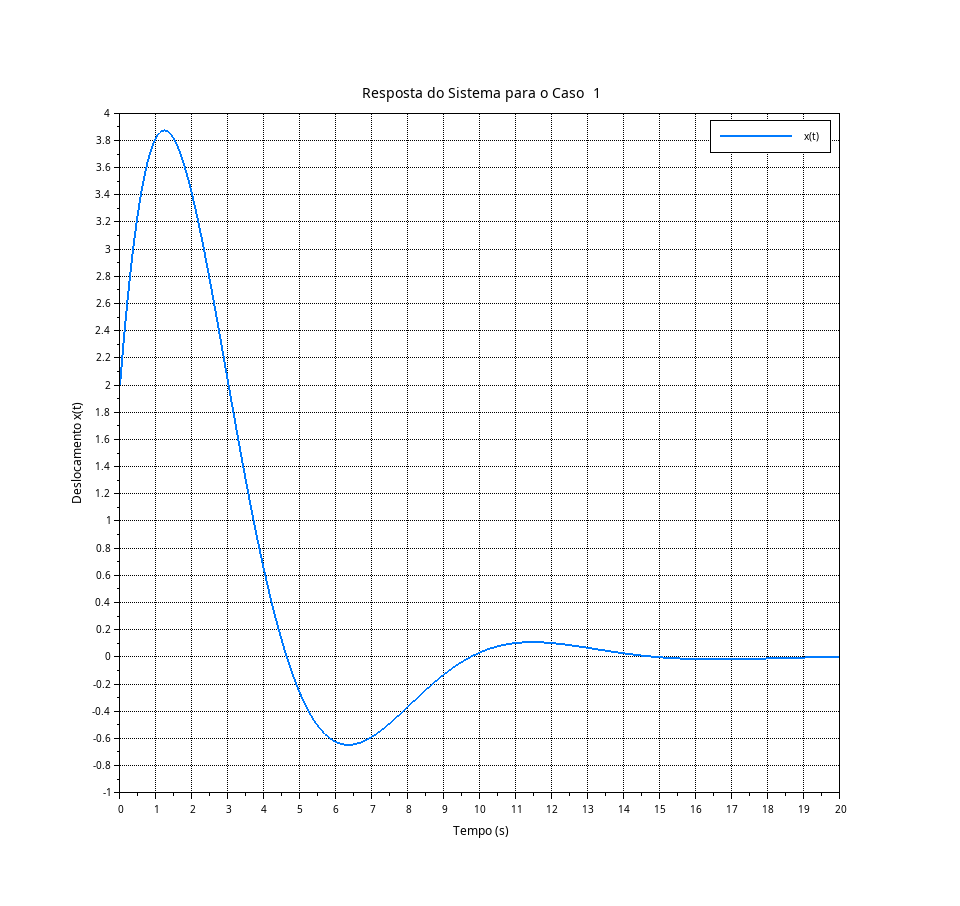
\includegraphics[width=0.6\textwidth]{final/1-atividade/assets/caso1.png}
    \caption{Resposta do sistema para o Caso 1}
\end{figure}
No Caso 1, o sistema é inicialmente impulsionado com uma alta velocidade (\(5 \, \text{m/s}\)), partindo do repouso (\(X_0 = 0\)). Esta condição inicial leva a uma resposta inicialmente enérgica, onde a massa oscila com uma amplitude elevada, seguida de um rápido decaimento energético devido ao amortecimento significativo (\(C = 7 \, \text{Ns/m}\)). O amortecimento não só reduz a amplitude das oscilações rapidamente, mas também garante que o sistema não persista em um estado de oscilação prolongada, estabilizando-se em um tempo curto.

\subsubsection{Caso 2: Deslocamento Inicial Sem Velocidade}
\begin{figure}[H]
    \centering
    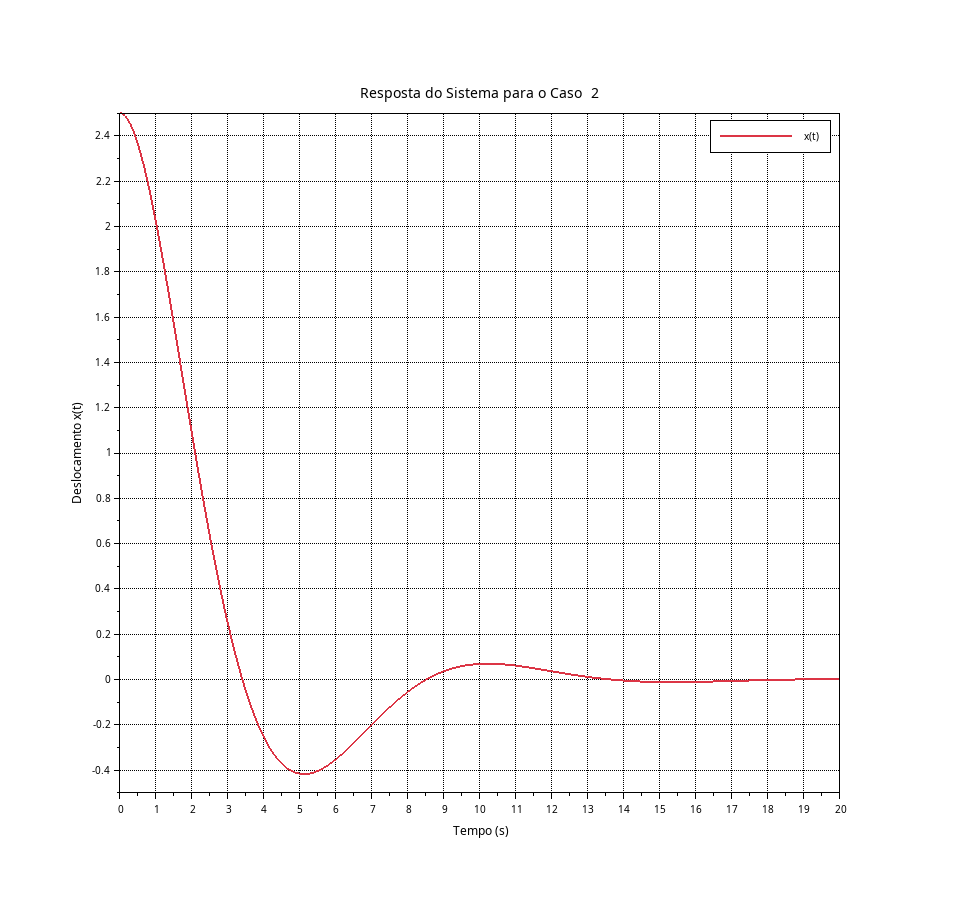
\includegraphics[width=0.6\textwidth]{final/1-atividade/assets/caso2.png}
    \caption{Resposta do sistema para o Caso 2}
\end{figure}
O Caso 2 é caracterizado por um deslocamento inicial (\(2.5 \, \text{m}\)) sem impulso inicial de velocidade (\(V_0 = 0\)). Aqui, observamos uma resposta típica de um sistema oscilatório subamortecido onde o sistema retorna ao equilíbrio através de oscilações que decaem gradativamente. Este caso destaca como a energia potencial armazenada na mola é convertida em energia cinética e dissipada pelo amortecedor. As oscilações decrescem em amplitude mais gradualmente do que no Caso 1, demonstrando uma transferência de energia mais prolongada antes da estabilização.

\subsubsection{Caso 3: Velocidade e Deslocamento Iniciais}
\begin{figure}[H]
    \centering
    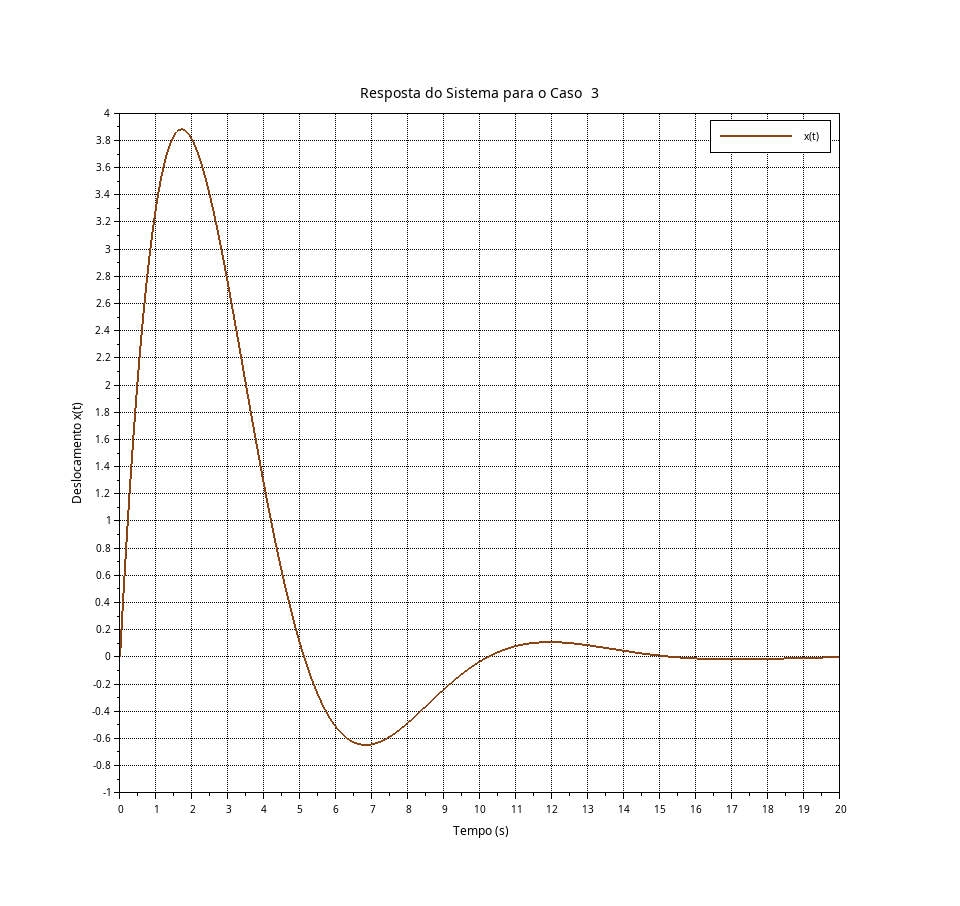
\includegraphics[width=0.6\textwidth]{final/1-atividade/assets/caso3.png}
    \caption{Resposta do sistema para o Caso 3}
\end{figure}
No Caso 3, o sistema inicia com condições iniciais moderadas tanto de velocidade (\(3.33 \, \text{m/s}\)) quanto de deslocamento (\(2 \, \text{m}\)). Esta configuração produz uma resposta dinâmica complexa, onde a interação entre energia cinética e potencial é mais evidente. A amplitude inicial é significativa, com uma taxa de decaimento que ilustra eficientemente o papel do amortecimento. As oscilações observadas são mais sustentadas que no Caso 1, mas menos intensas do que no Caso 2, refletindo um equilíbrio entre as energias cinética e potencial no início da simulação.

\subsubsection{Comparação Unificada dos Casos}
\begin{figure}[H]
    \centering
    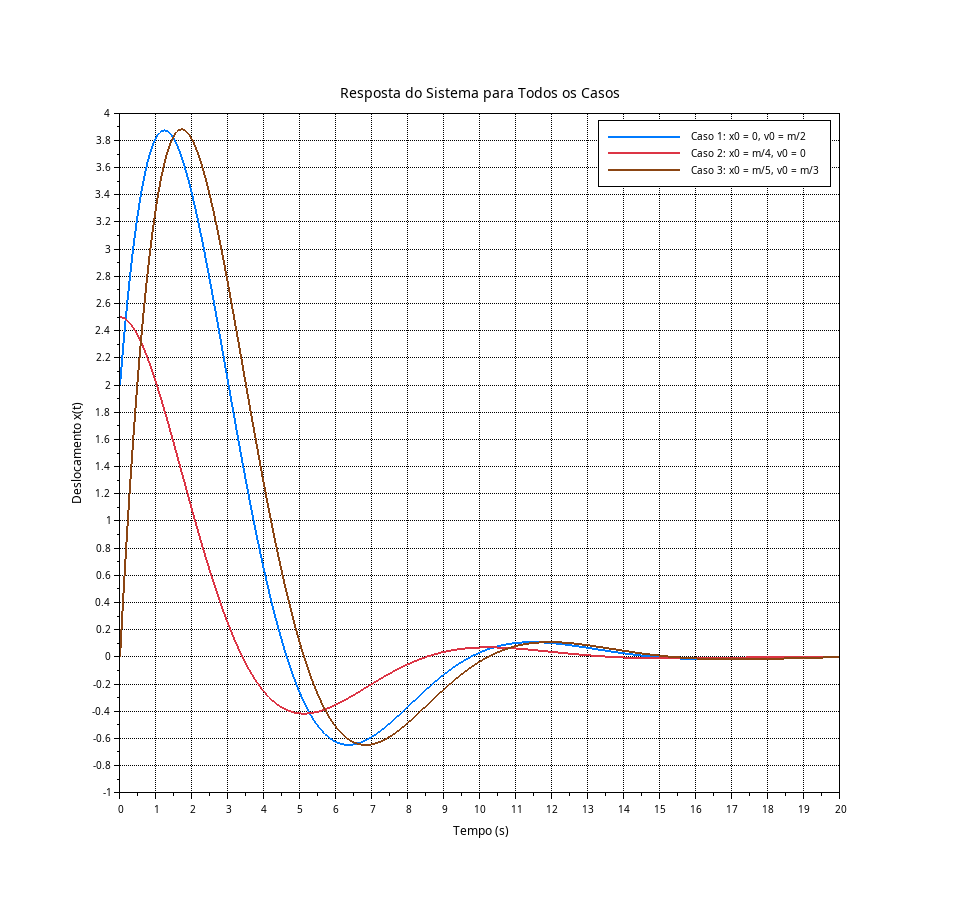
\includegraphics[width=0.6\textwidth]{final/1-atividade/assets/caso-all-in-one.png}
    \caption{Resposta unificada do sistema para os Casos 1, 2 e 3}
\end{figure}
A análise unificada dos três casos demonstra de forma clara as diferenças significativas nas respostas do sistema decorrentes de diversas condições iniciais. A seguir, discutiremos detalhadamente cada resposta e suas implicações para a compreensão do comportamento dinâmico do sistema:

\begin{itemize}
    \item \textbf{Caso 1 (Azul Escuro)}: Iniciado com uma alta velocidade inicial (\(5 \, \text{m/s}\)) e sem deslocamento inicial, este caso exibe a maior amplitude de oscilação observada. A energia cinética inicial é rapidamente convertida em energia potencial pela mola, resultando em oscilações de grande amplitude que são rapidamente amortecidas. Este caso ilustra o efeito de um forte amortecimento, onde a energia é dissipada rapidamente, levando a um retorno rápido à posição de equilíbrio sem oscilações residuais prolongadas. Esta configuração é ideal em situações onde a rápida estabilização após distúrbios é crucial, como em sistemas de suspensão de veículos.

    \item \textbf{Caso 2 (Vermelho)}: Com um deslocamento inicial (\(2.5 \, \text{m}\)) e sem velocidade inicial, o sistema mostra uma resposta clássica de um oscilador subamortecido. A energia potencial armazenada na mola é convertida gradualmente em energia cinética, com a energia sendo dissipada ao longo do tempo pelo amortecedor. As oscilações decaem suavemente, refletindo uma conversão mais lenta de energia que é típica em aplicações onde é necessário manter uma certa quantidade de movimento ou onde oscilações graduais são preferíveis, como em alguns tipos de sensores mecânicos.

    \item \textbf{Caso 3 (Marrom)}: Este caso combina condições iniciais moderadas de velocidade (\(3.33 \, \text{m/s}\)) e deslocamento (\(2 \, \text{m}\)), resultando numa resposta dinâmica mais complexa que engloba características dos dois primeiros casos. A amplitude inicial é significativa, mas as oscilações são mais controladas e decaem de maneira gradual. Este caso destaca a importância do equilíbrio entre rigidez da mola e amortecimento no projeto de sistemas mecânicos, onde é necessário um compromisso entre estabilidade rápida e manutenção de energia dinâmica.
\end{itemize}

Esta comparação detalhada destaca não apenas a influência das condições iniciais na resposta do sistema, mas também o papel crítico do amortecimento e da rigidez da mola na determinação da natureza da resposta dinâmica. A análise fornece insights valiosos para o design e a otimização de sistemas mecânicos em engenharia, sublinhando a necessidade de uma seleção cuidadosa de parâmetros de acordo com os requisitos específicos de cada aplicação.


\subsection{Comentários Gerais e Conclusão}
Os gráficos e análises ilustram claramente como as condições iniciais impactam a resposta dinâmica do sistema massa-mola-amortecedor. A energia inicial, seja como deslocamento ou velocidade, define a resposta imediata do sistema, mostrando a complexidade do comportamento de sistemas dinâmicos lineares. Observamos que o amortecimento é essencial para reduzir as oscilações e trazer o sistema de volta ao repouso de maneira eficiente, sublinhando sua importância no design de componentes mecânicos.

A adequação do coeficiente de amortecimento e da rigidez da mola é crucial para otimizar sistemas para suas funções específicas, como a absorção de choques em suspensões de veículos ou a precisão em instrumentos de medição. Além disso, a análise das condições iniciais é vital no planejamento e teste de sistemas mecânicos, onde engenheiros e designers devem antecipar cenários variados de operação.

Este estudo destaca a necessidade de um entendimento profundo das dinâmicas de sistemas para inovação em engenharia, proporcionando uma base sólida para a compreensão dos princípios de mecânica e dinâmica que são fundamentais no design de sistemas controlados e mecanismos em geral.

% \section{Atividade 2}

\subsection{Descrição do Modelo e Simulação}
Esta atividade envolve a criação de um diagrama de blocos no Xcos que simula a resposta de um sistema massa-mola-amortecedor com uma entrada especificada como \( f(t) = \frac{m}{5} \), onde \( m = 10 \) unidades de massa. O objetivo é analisar o comportamento do sistema sob diferentes condições iniciais e identificar métricas específicas do sistema dinâmico.

\subsection{Parâmetros do Sistema e Condições Iniciais}
Os parâmetros utilizados no modelo do sistema são:
\begin{itemize}
    \item Massa, \( m = 10 \) unidades.
    \item Coeficiente de amortecimento, \( C = 7 \) unidades.
    \item Constante da mola, \( k = 5 \) unidades.
\end{itemize}

A tabela a seguir detalha as condições iniciais ajustadas com base nos parâmetros do sistema:
\begin{center}
\begin{tabular}{|c|c|c|}
\hline
Caso & Velocidade Inicial \( V_0 \) & Posição Inicial \( X_0 \) \\
\hline
1 & \( 5 \, \text{m/s} \) (\( \frac{m}{2} \)) & \( 0 \, \text{m} \) \\
2 & \( 0 \, \text{m/s} \) & \( 2.5 \, \text{m} \) (\( \frac{m}{4} \)) \\
3 & \( 3.33 \, \text{m/s} \) (\( \frac{m}{3} \)) & \( 2 \, \text{m} \) (\( \frac{m}{5} \)) \\
\hline
\end{tabular}
\end{center}

Na verdade deixa quieto para essa atividade 1 não faz sentido o caso extra

Então vou manter os originais, te passar o tex base, as imagens geradas para sua analise e melhoria

\subsection{Resultados e Análise}
\subsubsection{Gráfico de Deslocamento}
\begin{figure}[H]
    \centering
    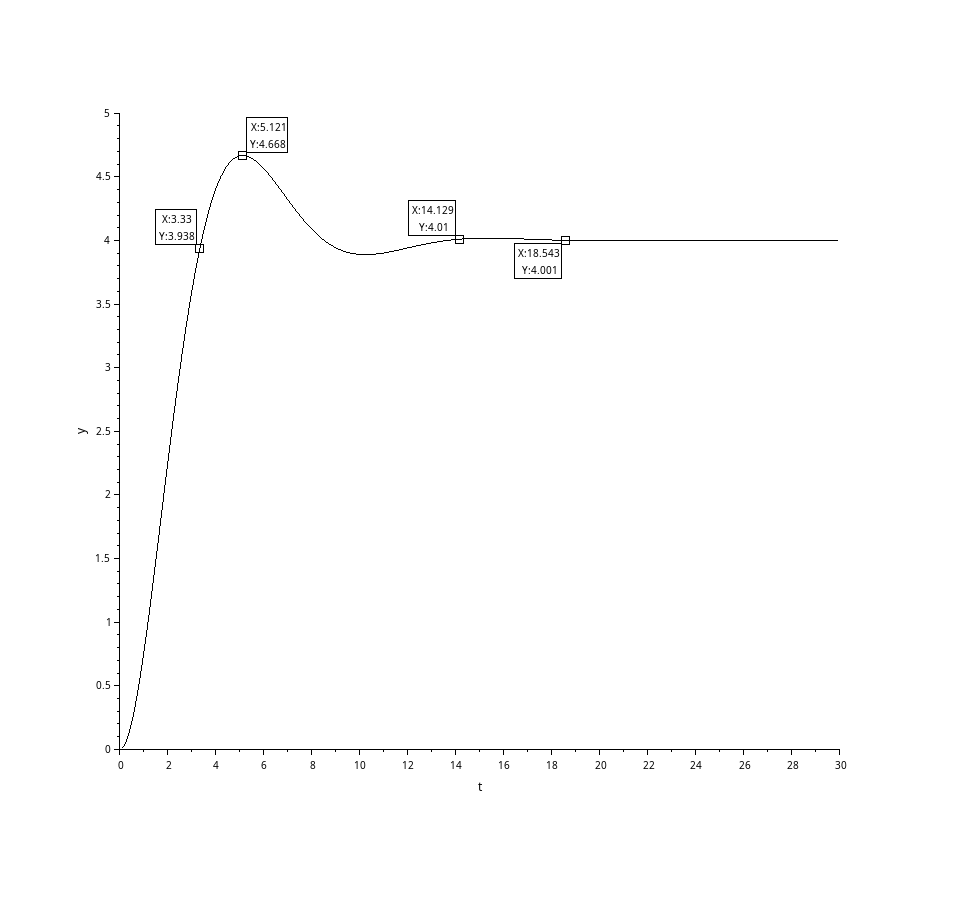
\includegraphics[width=0.7\textwidth]{2-atividade/xcos/deslocamento-caso-0.png}
    \caption{Gráfico de deslocamento com parâmetros comentados}
\end{figure}

\subsection{Resultados e Análise}
\subsubsection{Gráfico de Deslocamento}
\begin{figure}[H]
    \centering
    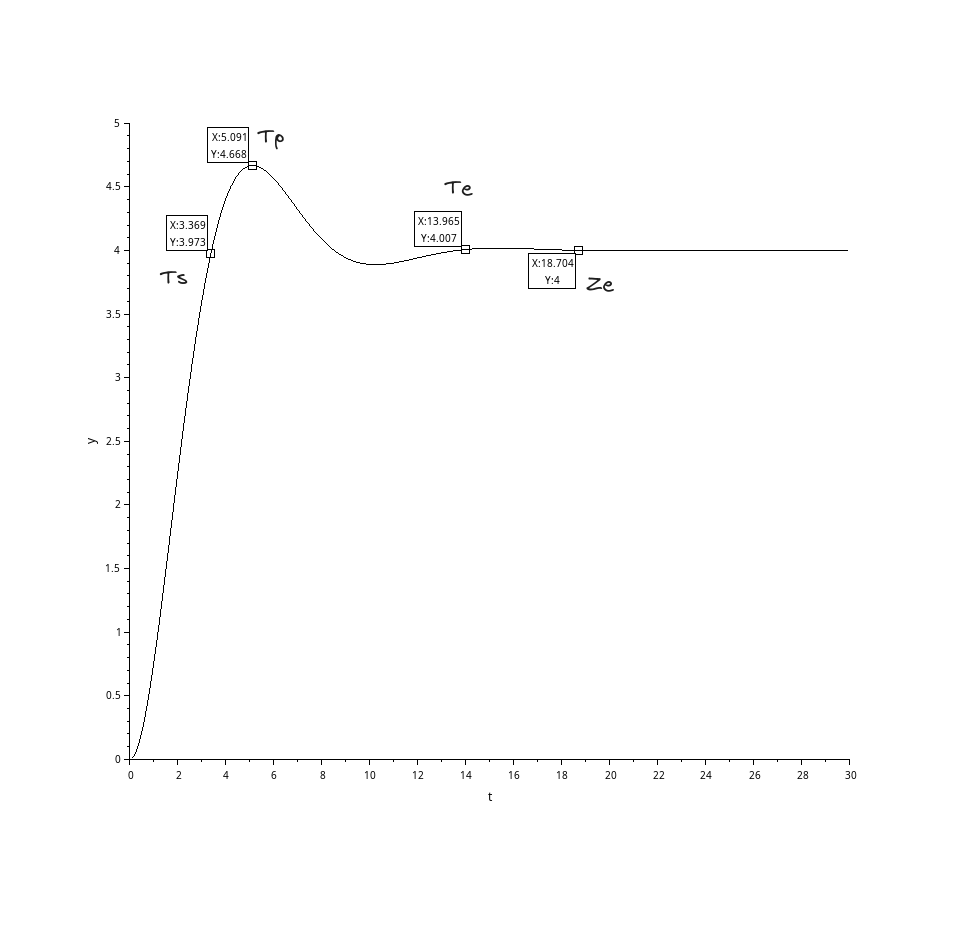
\includegraphics[width=0.7\textwidth]{2-atividade/assets/deslocamento-comentado.png}
    \caption{Gráfico de deslocamento com parâmetros comentados}
\end{figure}
No gráfico de deslocamento, são identificados os seguintes pontos:
\begin{itemize}
    \item \textbf{Tempo de Subida (Ts)}: Tempo necessário para o deslocamento alcançar pela primeira vez o seu valor máximo.
    \item \textbf{Tempo de Pico (Tp)}: Momento em que o deslocamento atinge o seu valor máximo.
    \item \textbf{Tempo de Estabelecimento (Te)}: Tempo necessário para que o deslocamento se estabilize dentro de uma faixa aceitável em torno do valor final.
    \item \textbf{Zona Estacionária (Ze)}: Região no gráfico onde o sistema mantém um comportamento constante, indicando o estado estacionário.
\end{itemize}

\subsubsection{Gráfico de Velocidade}
\begin{figure}[H]
    \centering
    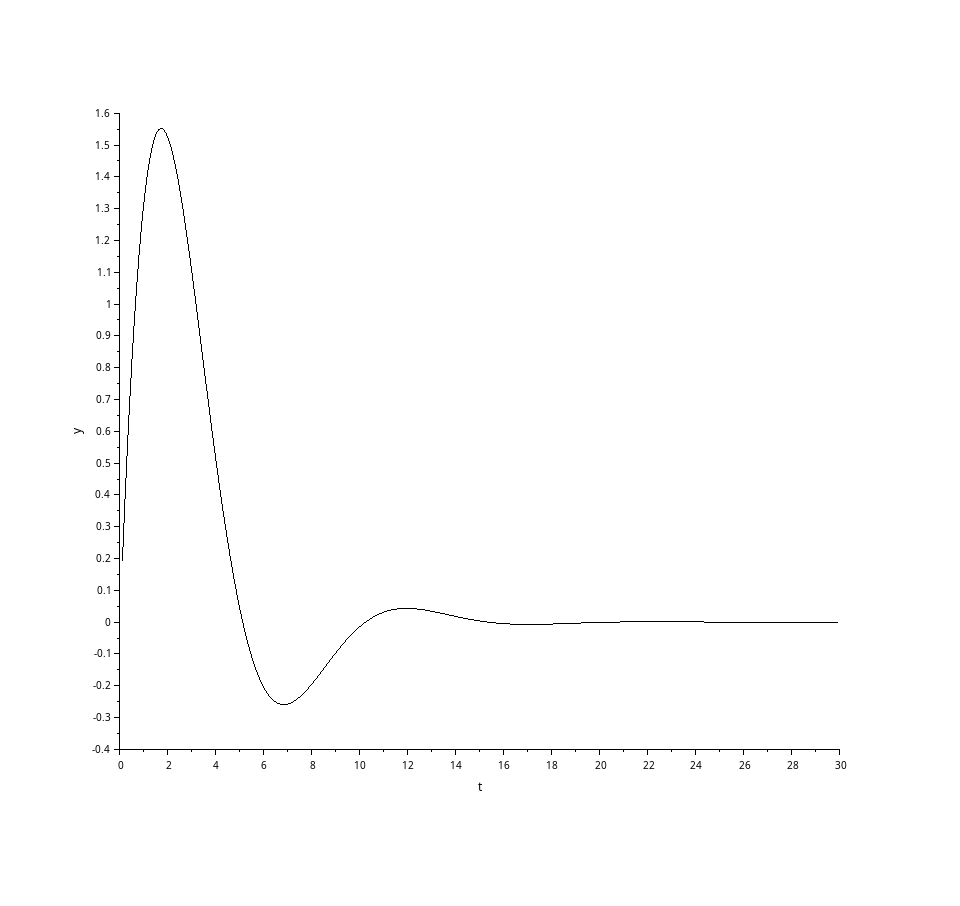
\includegraphics[width=0.7\textwidth]{2-atividade/assets/velocidade.png}
    \caption{Gráfico de velocidade}
\end{figure}
O gráfico de velocidade fornece uma visão sobre como a velocidade do sistema varia ao longo do tempo em resposta à entrada aplicada e às condições iniciais.

\subsection{Conclusões}
A análise dos gráficos de deslocamento e velocidade mostra a eficácia do amortecimento e a influência da rigidez da mola nas respostas do sistema. Cada caso demonstra um comportamento único que é crucial para entender a dinâmica do sistema sob várias condições iniciais.

% \section{Atividade 3}

\subsection{Descrição do Modelo e Análise de Sistema}
Nesta atividade, foi desenvolvida a função de transferência para um sistema massa-mola-amortecedor com os seguintes parâmetros específicos para o estudante Guilherme Cagide Fialho:
\begin{itemize}
    \item Massa, \( m = 10 \) kg.
    \item Coeficiente de amortecimento, \( C = 7 \) Ns/m.
    \item Constante da mola, \( K = 5 \) N/m.
\end{itemize}
A função de transferência obtida é:
\[
G(s) = \frac{1}{10s^2 + 7s + 5}
\]

\subsection{Cálculo dos Polos e Parâmetros do Sistema}
Os polos da função de transferência são complexos conjugados e foram calculados como:
\begin{itemize}
    \item Polo 1: \( -0.35 + 0.614j \)
    \item Polo 2: \( -0.35 - 0.614j \)
\end{itemize}

Os parâmetros típicos do sistema de segunda ordem são:
\begin{itemize}
    \item Frequência natural não-amortecida (\( \omega_n \)): \( 0.707 \) rad/s
    \item Coeficiente de amortecimento (\( \zeta \)): \( 0.495 \)
    \item Ganho estático (\( K_p \)): \( 0.2 \)
\end{itemize}

\subsection{Resposta ao Impulso}
A resposta ao impulso do sistema foi simulada e é mostrada na figura abaixo:
\begin{figure}[H]
    \centering
    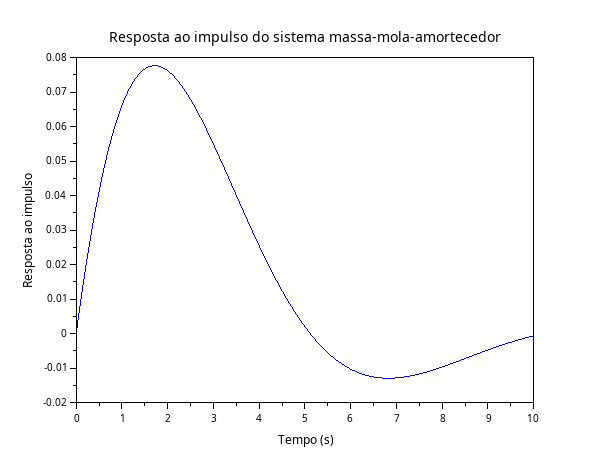
\includegraphics[width=0.8\textwidth]{3-atividade/assets/resposta-ao-impulso.png}
    \caption{Resposta ao impulso do sistema massa-mola-amortecedor}
\end{figure}

\subsection{Discussão}
A análise dos polos mostra que o sistema é subamortecido, o que é corroborado pelo coeficiente de amortecimento menor que 1. A resposta ao impulso ilustra um comportamento oscilatório decaído, típico de sistemas subamortecidos, onde as oscilações diminuem gradualmente até a estabilização. O ganho estático (\( K_p \)) indica a resposta do sistema a uma entrada de degrau unitário em regime permanente.

\subsection{Conclusões}
A simulação e os cálculos realizados fornecem uma visão detalhada da dinâmica do sistema, evidenciando como os parâmetros de massa, amortecimento e rigidez influenciam o comportamento do sistema. Esta análise é essencial para o entendimento e design de sistemas de controle que possam efetivamente gerenciar tais dinâmicas.

% \section{Atividade 4}

\subsection{Descrição do Modelo e Simulação}
Nesta atividade, analisamos um sistema de controle típico. Utilizamos um controlador proporcional cujo ganho \( K \) é determinado pela relação \( \frac{m}{3} \), onde \( m \) é a massa do sistema. A função de transferência da planta (Gp) é derivada da equação dinâmica da massa, amortecimento e constante da mola, especificada na Atividade 3. O sensor é modelado por um sistema de primeira ordem, com ganho unitário \( K_s = 1 \) e constante de tempo \( T_s = \frac{m}{6} \).

\subsection{Construção do Diagrama de Blocos}
Abaixo, apresentamos o diagrama de blocos para o sistema de controle, ilustrando a interação entre o controlador, a planta e o sensor.

\begin{figure}[H]
    \centering
    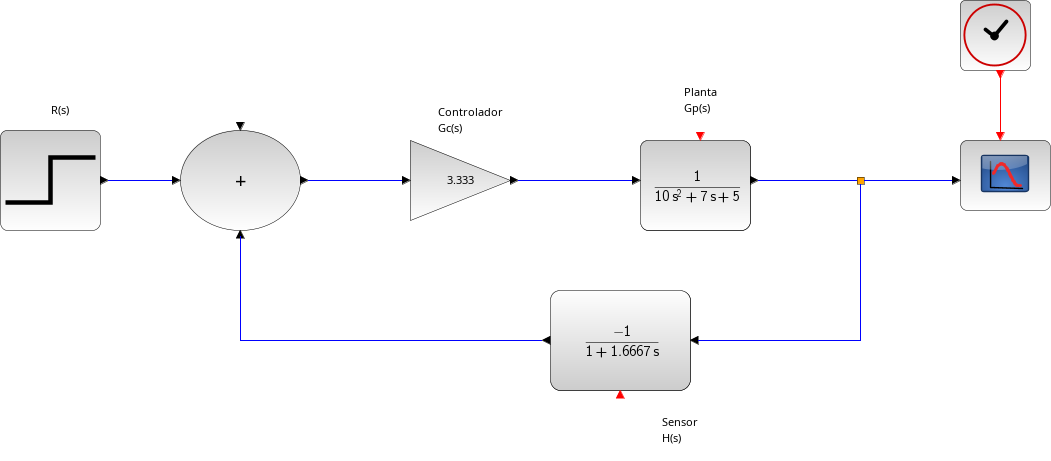
\includegraphics[width=0.7\textwidth]{4-atividade/assets/diagrama-blocos.png}
    \caption{Diagrama de blocos do sistema de controle}
    \label{fig:diagrama_blocos}
\end{figure}

As funções de transferência são especificadas como segue:
\begin{itemize}
    \item Controlador: \( G_c(s) = \frac{m}{3} \) com \( m = 10 \), então \( G_c(s) = \frac{10}{3} \)
    \item Planta: \( G_p(s) = \frac{1}{m s^2 + C s + K} = \frac{1}{10 s^2 + 7 s + 5} \)
    \item Sensor: \( H(s) = \frac{1}{1 + \frac{m}{6} s} = \frac{1}{1 + 1.6667 s} \)
\end{itemize}

\subsection{Função de Transferência em Malha Fechada}
Calculamos a função de transferência em malha fechada \( C(s)/R(s) \) pela fórmula:
\[
    G_{closed}(s) = \frac{G_c(s) \cdot G_p(s)}{1 + G_c(s) \cdot G_p(s) \cdot H(s)}
\]
Substituímos as funções de transferência obtidas:
\[
    G_{closed}(s) = \frac{\frac{10}{3} \cdot \frac{1}{10 s^2 + 7 s + 5}}{1 + \frac{10}{3} \cdot \frac{1}{10 s^2 + 7 s + 5} \cdot \frac{1}{1 + 1.6667 s}}
\]
Simplificamos a expressão para chegar à forma final da função de transferência em malha fechada:
\[
    G_{closed}(s) = \frac{0.3333333s + 0.2}{s^3 + 1.3s^2 + 0.92s + 0.5}
\]

\subsection{Análise de Estabilidade pelo Critério de Routh-Hurwitz}
Utilizamos o critério de Routh-Hurwitz para avaliar a estabilidade do sistema, baseando-nos nos coeficientes do denominador da função de transferência em malha fechada.

\subsubsection{Resultados da Análise de Estabilidade}
A matriz de Routh-Hurwitz, obtida a partir dos coeficientes do polinômio do denominador, é apresentada a seguir:
\[
    RH\_matrix = \begin{bmatrix}
        0.5  & ... \\
        0.92 & ... \\
        1.3  & ... \\
        1    & ... \\
    \end{bmatrix}
\]
O sistema é considerado estável, pois todos os elementos da primeira coluna são positivos.

\subsection{Análise de Estabilidade para Diferentes Valores de \( K \)}
Investigamos a estabilidade do sistema para diferentes valores do ganho do controlador \( K_p \), variando de 1 a 10. As análises mostram que o sistema mantém a estabilidade em todo o intervalo testado.

\subsubsection{Resultados da Resposta ao Degrau}
Abaixo, apresentamos o gráfico da resposta ao degrau para os diferentes valores de \( K_p \):

\begin{figure}[H]
    \centering
    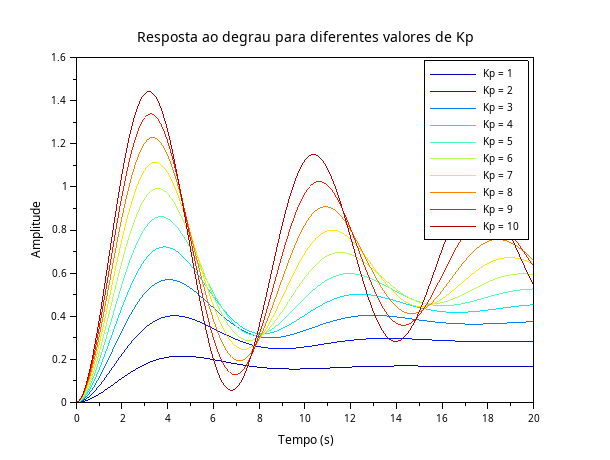
\includegraphics[width=0.7\textwidth]{4-atividade/assets/impulsos-diferentes-kp.png}
    \caption{Resposta ao degrau para diferentes valores de \( K_p \)}
    \label{fig:resposta-degrau-kp}
\end{figure}

\subsection{Conclusões}
As análises mostram que o sistema massa-mola-amortecedor controlado proporcionalmente é estável para os valores de \( K_p \) entre 1 e 10. Observa-se que o comportamento da resposta ao degrau varia significativamente com o ganho do controlador, destacando a necessidade de ajuste adequado para alcançar a resposta desejada do sistema.


\end{document}
